\chapter{Results and Discussion}
\label{cha:results}
\section{Numerical Tests in an 2D Toy Potential}
\label{sec:2D}
As a simple test to check all ABM methods a single particle in the two-dimensional potential $U_2$ (eq.~\ref{eq:U2}) is considered.
By performing a simple 2D to 2D mapping in the absence of any dimensionality reduction, the analytical PMF and free energy difference is given by
\begin{equation}
  \begin{split}
    A(x,y)&=U_2(x,y) \\
    \Delta A_{A\to B} &= 0
  \end{split}
\end{equation}
The convergence of numerical PMFs and free energy differences to the analytical result with different adaptive biasing schemes (MtD, WTM, ABF, eABF and WTM-eABF) is computed over the course of 5~ns trajectories.
Note that all adaptive biasing methods depend on a different set of parameters.
Their convergence can therefore only be compared qualitatively.
A detailed analysis of the impact of the choice of parameters will be given in the following section.
Parameters applied in this section and resulting PMFs after 1, 3 and 5~ns are given in the Appendix.
In Fig.~\ref{fig:conv 2D} the convergence of the PMF and corresponding estimate for the free energy difference over time is given.
Fig.~\ref{fig:error 2D} shows remaining absolute local errors at the end of all simulations.

In an unbiased simulation the system stays trapped in one metastable state.
This is a example of quasi-nonergodic behavior, where simple time averages of MD trajectories do not converge to the correct ensemble average.
Because only a small region of CV space is explored the free energy difference $\Delta A_{A\to B}$ is highly overestimated.

All adaptive biasing methods reduce the metastability significantly and enable uniform sampling of both states.
In MtD/WTM simulations the PMF is given by a superposition of Gaussian hills, which are deposited linearly over time and fill both minima consecutively.
For this particular set of parameters no full convergence is reached in 5~ns.
Regions with high free energy at the margins remain unexplored due to incomplete filling of the PMF with Gaussians and the obtained PMFs deviate from the analytic result by about 20~\%.
However, using WTM this is intentional as the fraction of the PMF that is compensated in the simulation is chosen with the effective temperature $\Delta T$.
The height of Gaussians is reduced over time, which results in significantly smaller fluctuations and absolute errors of the PMF in large parts of the PMF than with MtD.
After 4~ns the free energy difference $\Delta A_{A\to B}$ obtained from WTM therefore converges safely towards 0~kJ/mol.
\begin{figure}[H]
   \centering
   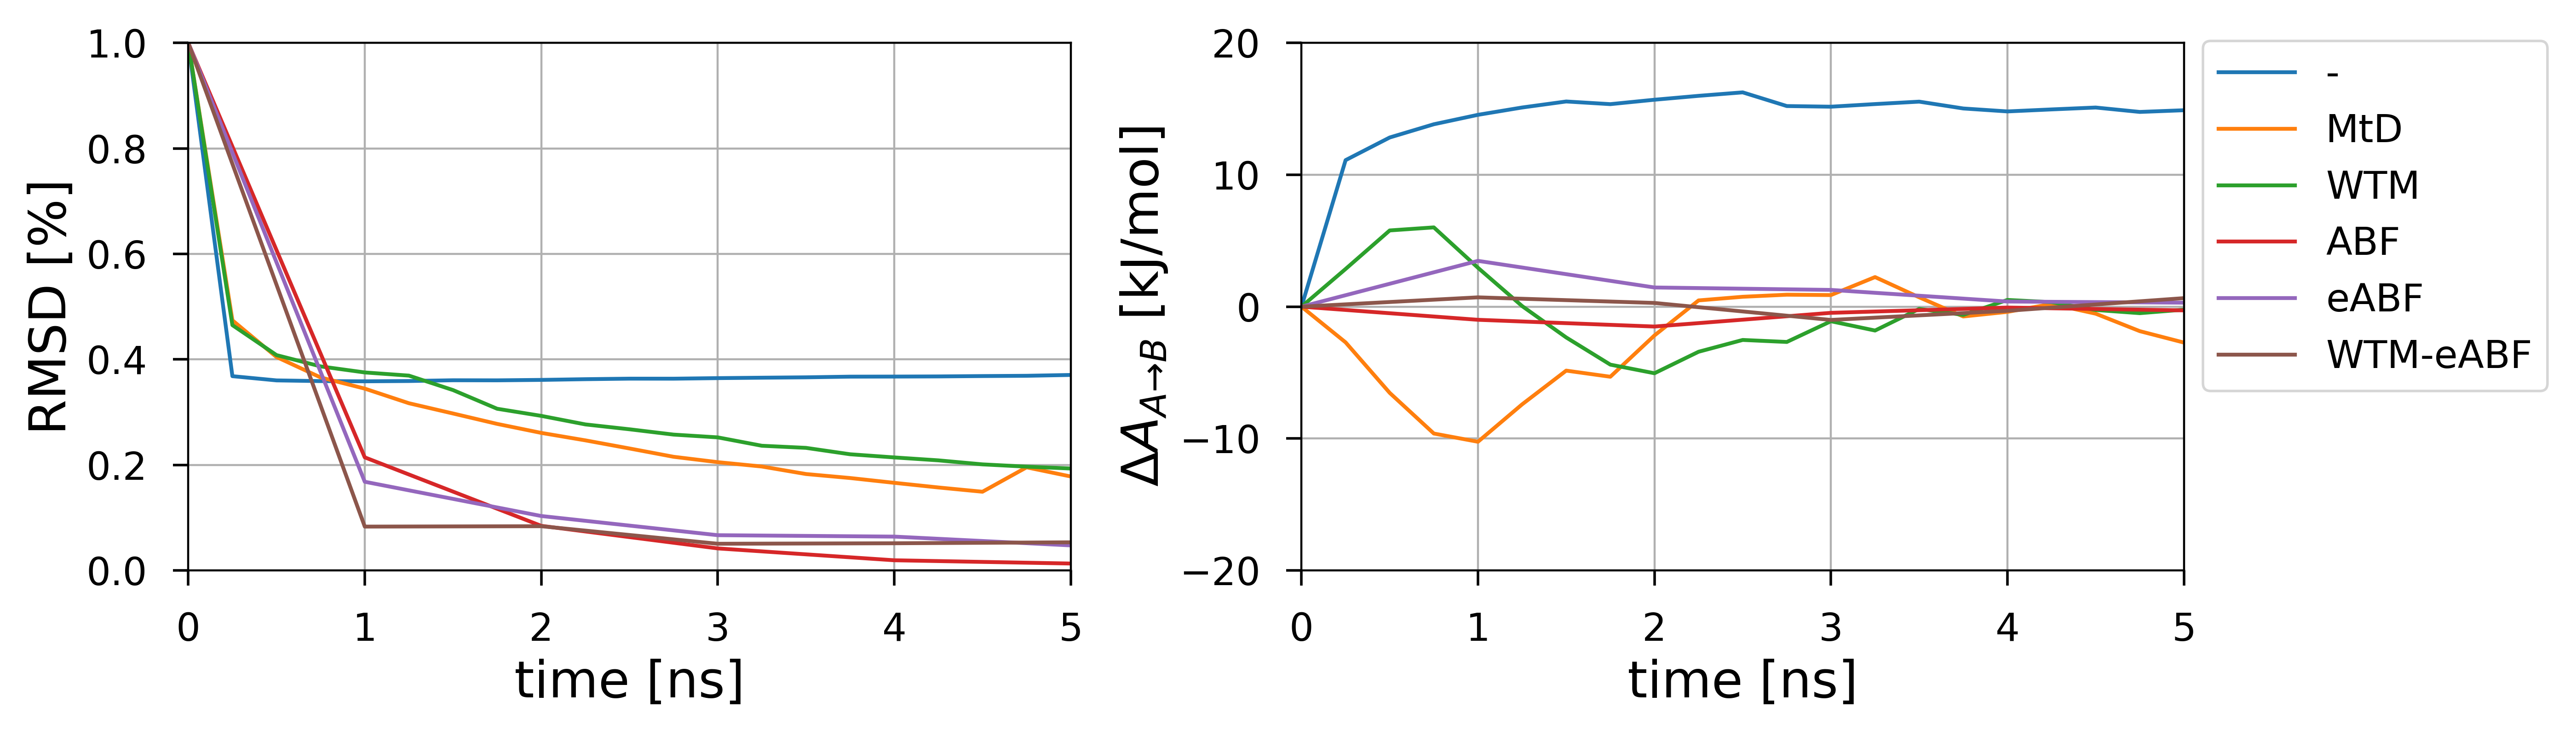
\includegraphics[width=0.99\textwidth]{bilder/test_2D/conv}
   \caption{Convergence of free energy calculations with different adaptive biasing methods for a 2D to 2D mapping of toy potential $U_2$. On the right the RMSD between the analytical and numerical PMF is given over the course of 5~ns trajectories. On the right the development of free energy differences $\Delta A_{A\to B}$ given by eq.~\ref{eq:free energy diff} is shown. Both metastable states are separated by the line $0.25x+y$. Therefore $A$ includes all states $x>-4y$ and $B$ all states $x<-4y$, respectively.}
 \label{fig:conv 2D}%
\end{figure}
\begin{figure}[H]
  \centering
  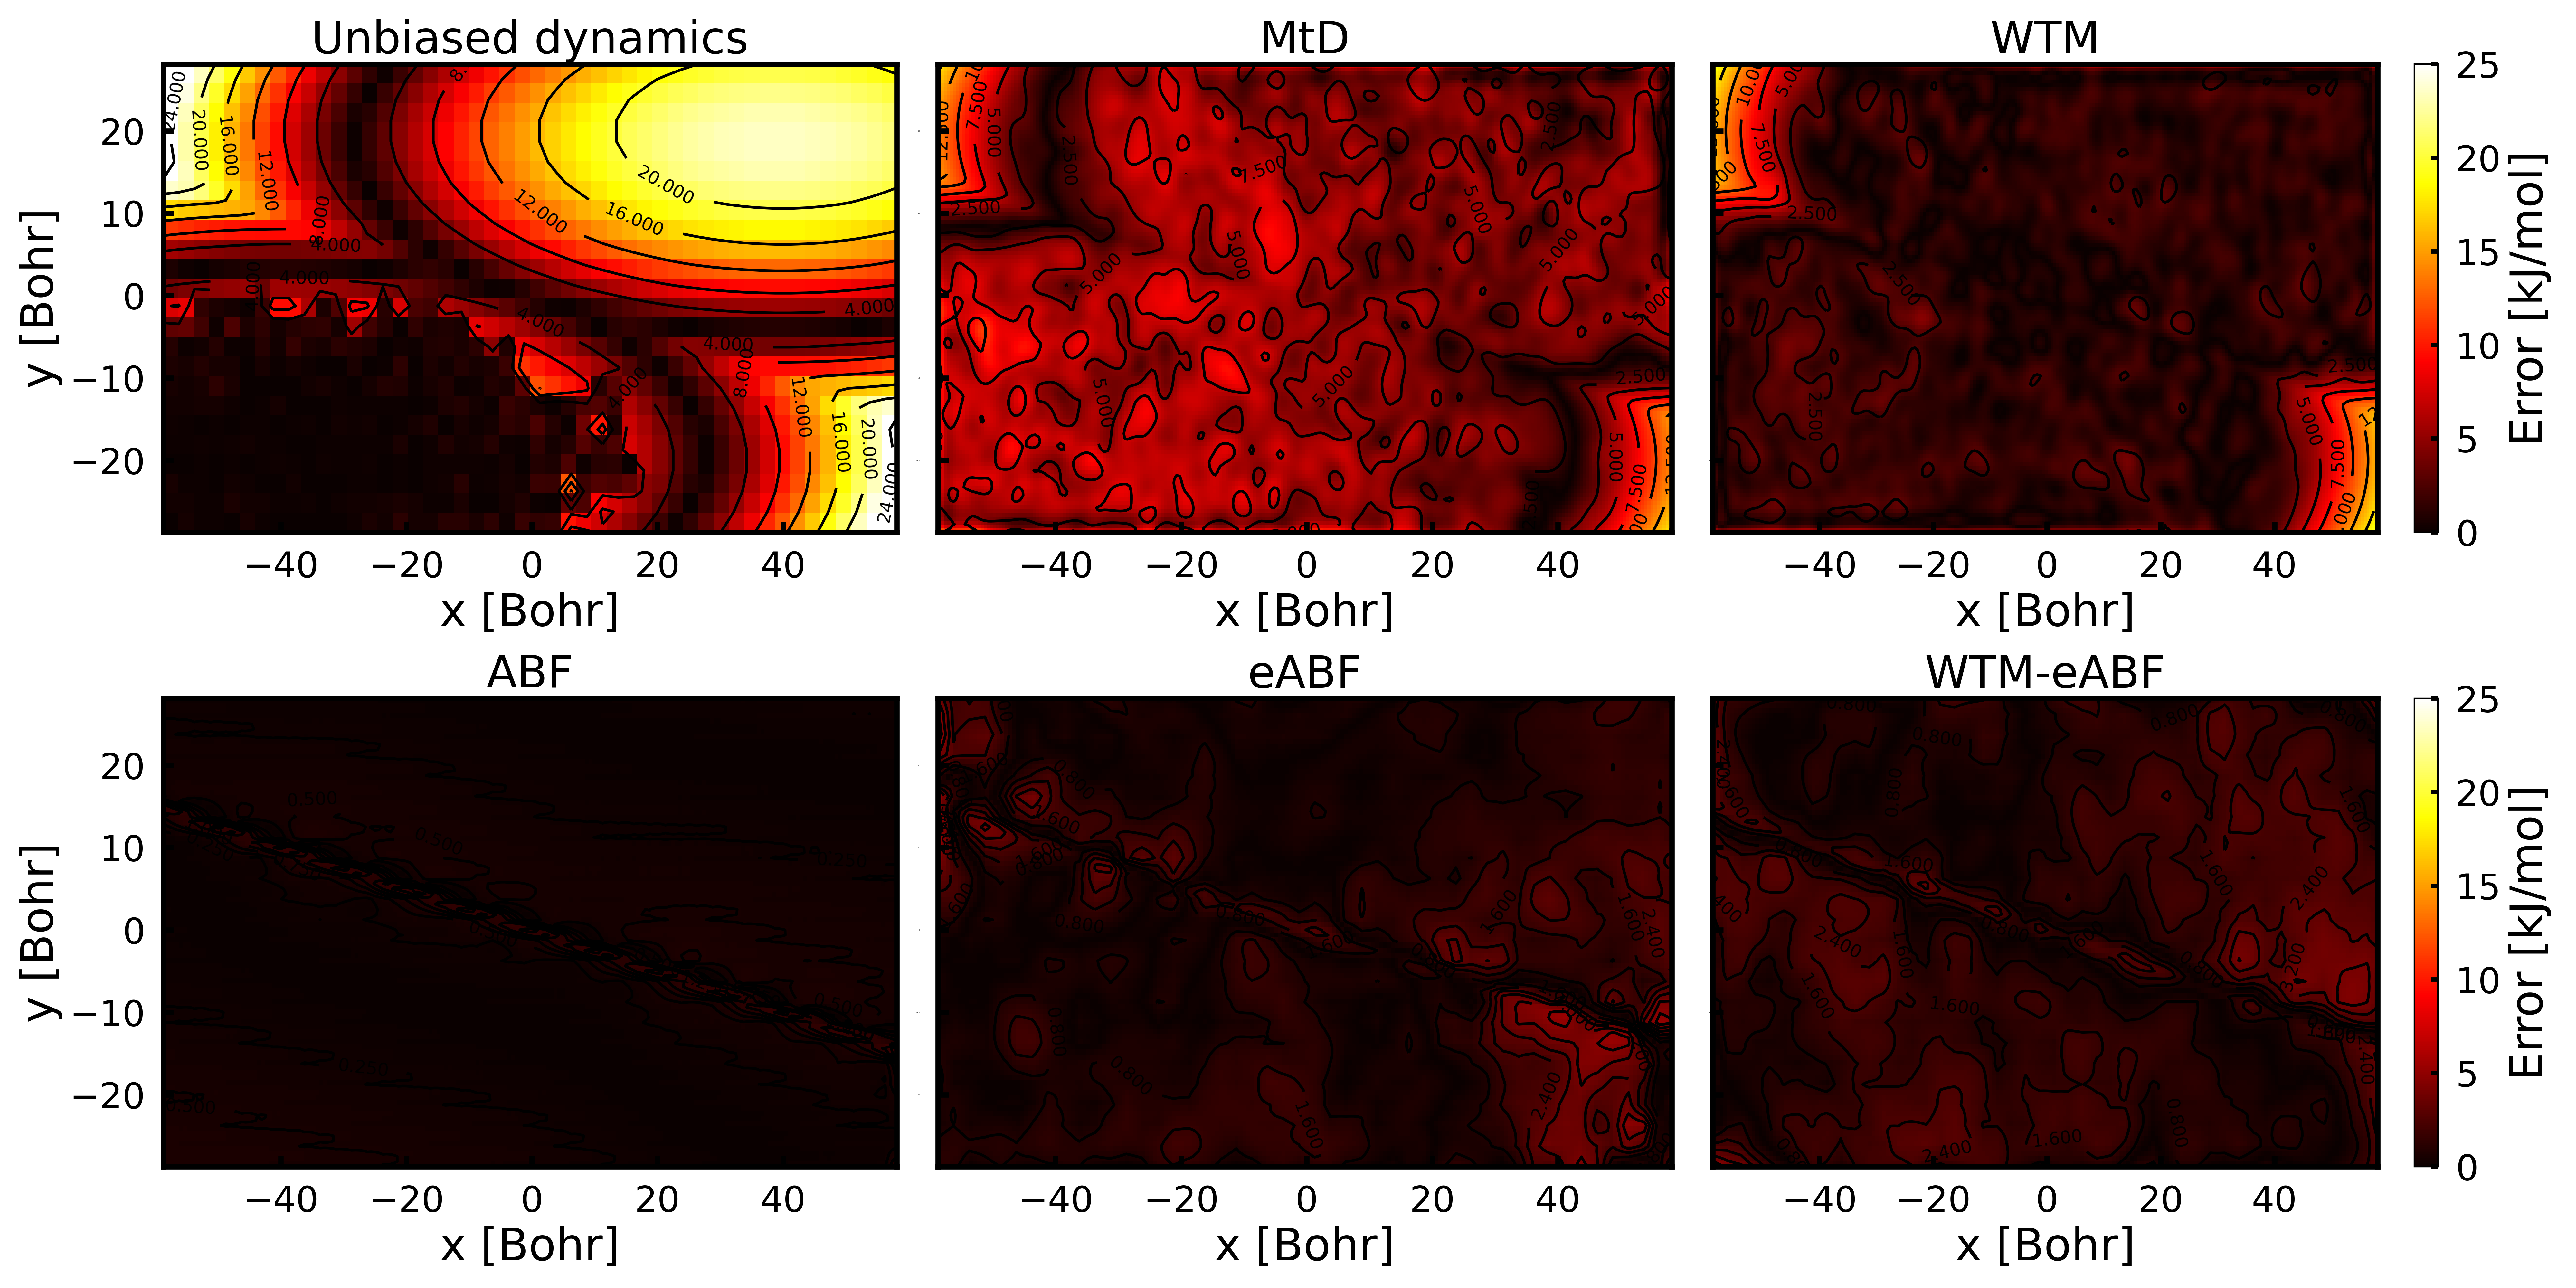
\includegraphics[width=0.99\textwidth]{bilder/test_2D/error_5ns}
  \caption{Heat maps of the absolute difference between the analytic and numerical PMFs. Numerical PMFs are obtained from 5~ns MD trajectories at 300~K.}
\label{fig:error 2D}%
\end{figure}
With ABF after 3~ns the potential is mapped almost perfectly with maximum local errors below 1~kJ/mol. Also the RMSD of the PMF and free energy difference $\Delta A_{A\to B}$ converges rigorously to the analytic results.
For this particular example ABF force samples are simply given by the gradient of the analytical potential.
The variance of force samples, which is only introduced by the finite bin width, is therefore small and convergence of the ABF force in individual bins is reached almost instantly.
Even faster exploration of the PMF is only hindered by the ramp function, which is not strictly necessary for this toy example, but still applied to provide a more realistic test case for real chemical applications.
PMFs are obtained by thermodynamic integration of ABF forces with the FEM method, as shown in Fig.~\ref{fig:ti}.
\begin{figure}[H]
  \centering
  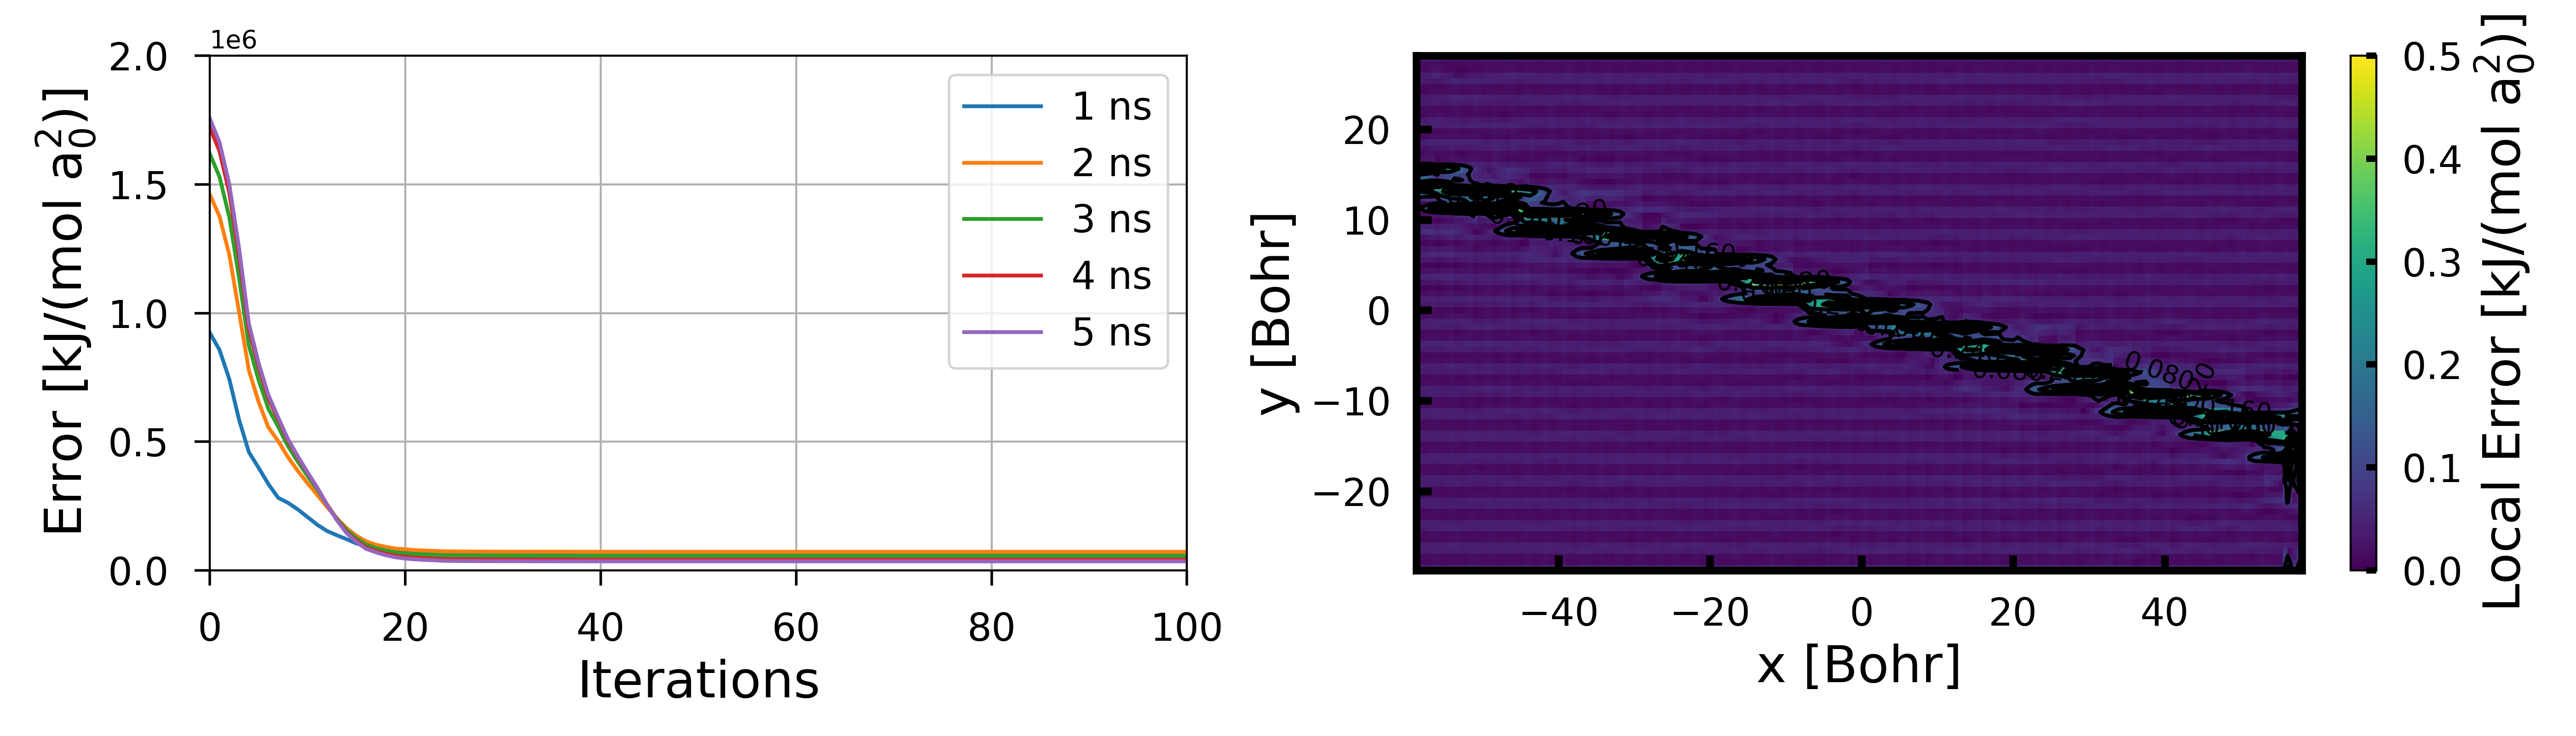
\includegraphics[width=0.99\textwidth]{bilder/test_2D/ti}
  \caption{On the left the convergence of the thermodynamic integration of ABF forces with the FEM method in a BFGS minimization is given. On the right the resulting mean local difference of optimized B-splines to the ABF forces is shown.}
\label{fig:ti}%
\end{figure}
Convergence of the FEM method is reached reliably in 100 iterations by minimization of eq.~\ref{eq:RMSD} with the BFGS algorithm.
At the transition barrier, where the thermodynamic force changes rapidly, this introduces small errors to the PMF, which can be reduced with a smaller bin width and more B-spline functions.

Both eABF and WTM-eABF preserve the rigorous convergence behavior of ABF.
By estimating the thermodynamic force over the extended-system, the variance of obtained force samples depends on the harmonic force constant of the coupling of the fictitious to the physical particle.
For this toy example this introduces some noise to the mean force, where it would reduce said noise in real chemical applications.\autocite{lesage2017smoothed}
The PMF therefore shows small fluctuations of up to 2~kJ/mol for both methods and convergence to the true PMF is reached with a final RMSD of about 2~\%.
However, quite surprisingly convergence of the mean force with eABF is as fast as with ABF and WTM-eABF gives an additional speed up.
With WTM-eABF the estimate for the free energy difference stays close to 0~kJ/mol over the course of the hole simulation.
This indicates that the hole PMF is explored uniformly from the beginning and the system is never trapped in one state.

In this section the favorable convergence behavior of ABF, eABF and WTM-eABF was demonstrated.
In the following sections this methods will be discussed in further detail for a real chemical system with special focus on the influence of input parameters on the simulations.

\newpage
\section{Benchmark Calculations for the Torsion of Cl-F-Ethane}
\label{sec:test}
The following section will give a detailed discussion on the effect of different parameters on the time convergence of adaptive biasing force methods (ABF, eABF and WTM-eABF).
As test system the transition of the dihedral angle between the Cl- and F-group in Cl-F-Ethane from the gauge$^+$ ($60^\circ$) to the gauge$^-$ ($-60^\circ$) structure on the PBEh-3c/dev2-msvp level of theory in vacuum will be considered.

Figure~\ref{fig:ABF benchmark} shows the PMF obtained from a ABF calculation for growing values of $N_{full}$ from 50~ps long trajectories.
Convergence rates will be calculated in reference to the ABF ($N_{full}=100$) result after 50~ps.
After roughly 30~ps all three simulations converge to the same result.
For higher values of $N_{full}$ it takes longer to fill the ramp functions.
Diffusion to other minima along the reaction coordinate and its uniform sampling is therefore delayed and convergence slowed down.
In this particular example, even the unrestrained application of the ABF force from the start ($N_{full}=1$) does not lead to any non-equilibrium effects.
However, as instantaneous force samples depend on all molecular coordinates, the variance of fluctuations in ABF estimates can be expected to grow with the system size.
More specifically fluctuations of the ABF force will be dominated by high frequency terms due to bonded interactions\autocite{lesage2017smoothed}, which also leads to a dependence of the variance in ABF force samples at the beginning of the simulation on the amount of equillibration.\autocite{blondel2004ensemble}
Using smaller values of $N_{full}$ is therefore associated with a certain risk to drive the system away from thermal equilibrium at the beginning of the simulation.
Correcting wrong force estimates obtained with high statistical weight at the beginning of the simulation takes exceedingly long which makes corresponding free energy estimates prone to errors.\autocite{comer2015adaptive}
Overall $N_{full}=100$ is found to result in a good compromise between save and fast convergence of the ABF force estimates for all systems considered in this work.
\begin{figure}[H]
    \centering
    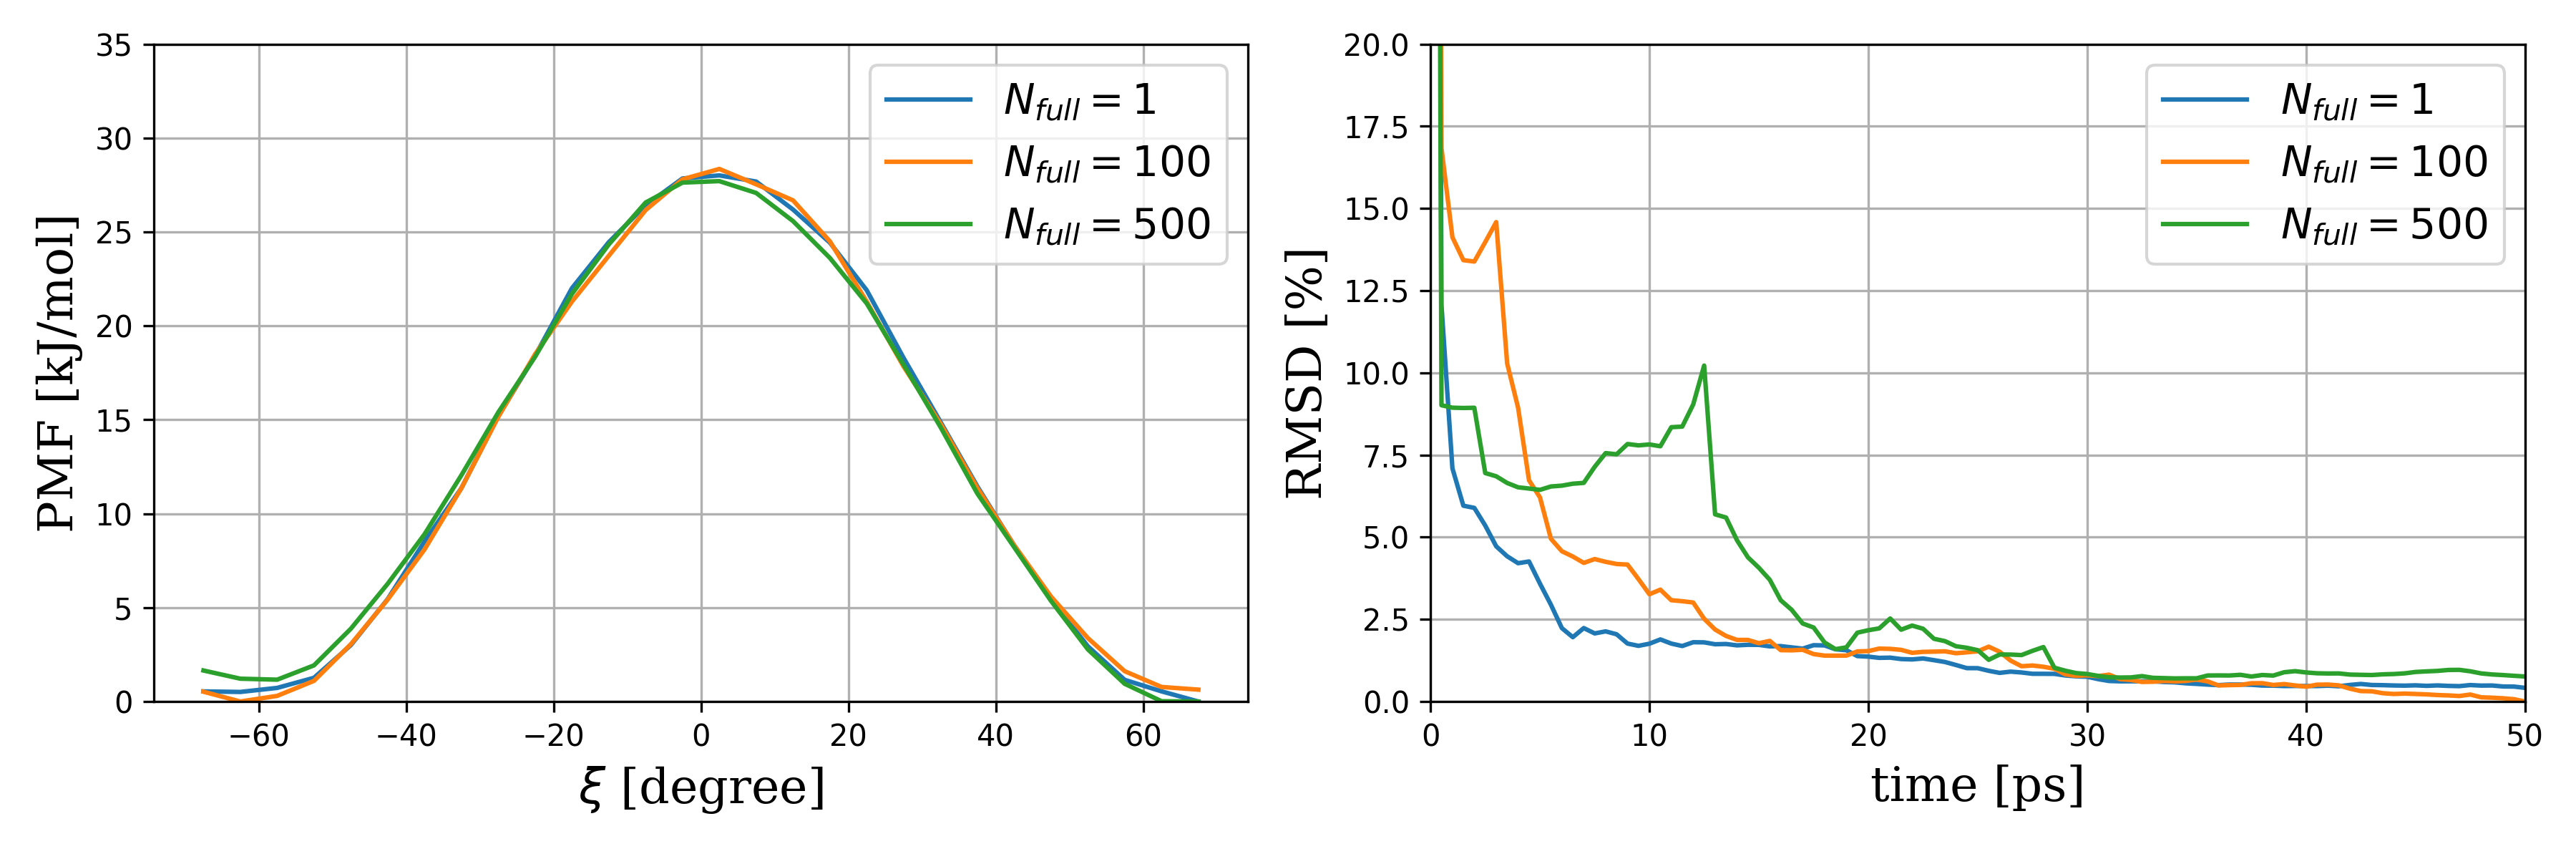
\includegraphics[width=0.99\textwidth]{bilder/benchmark/ABF_benchmark_nfull}
    \caption{ABF benchmark}
    \label{fig:ABF benchmark}
\end{figure}
For eABF the ramp function is applied in the exact same way and with the same consequences than for ABF.\autocite{lesage2017smoothed}
However, mean square fluctuations $\sigma_F$ of the eABF force only depend on the spring force between the CV and the extended variable and is therefore proportional to the harmonic force constant $k_\lambda$.
\begin{equation}
    \sigma_F^2 \propto \frac{k_\lambda}{\beta} = \frac{1}{\beta\sigma_\lambda}
\end{equation}
This implies that in eABF calculations higher the variance of
\begin{figure}[H]
  \centering
    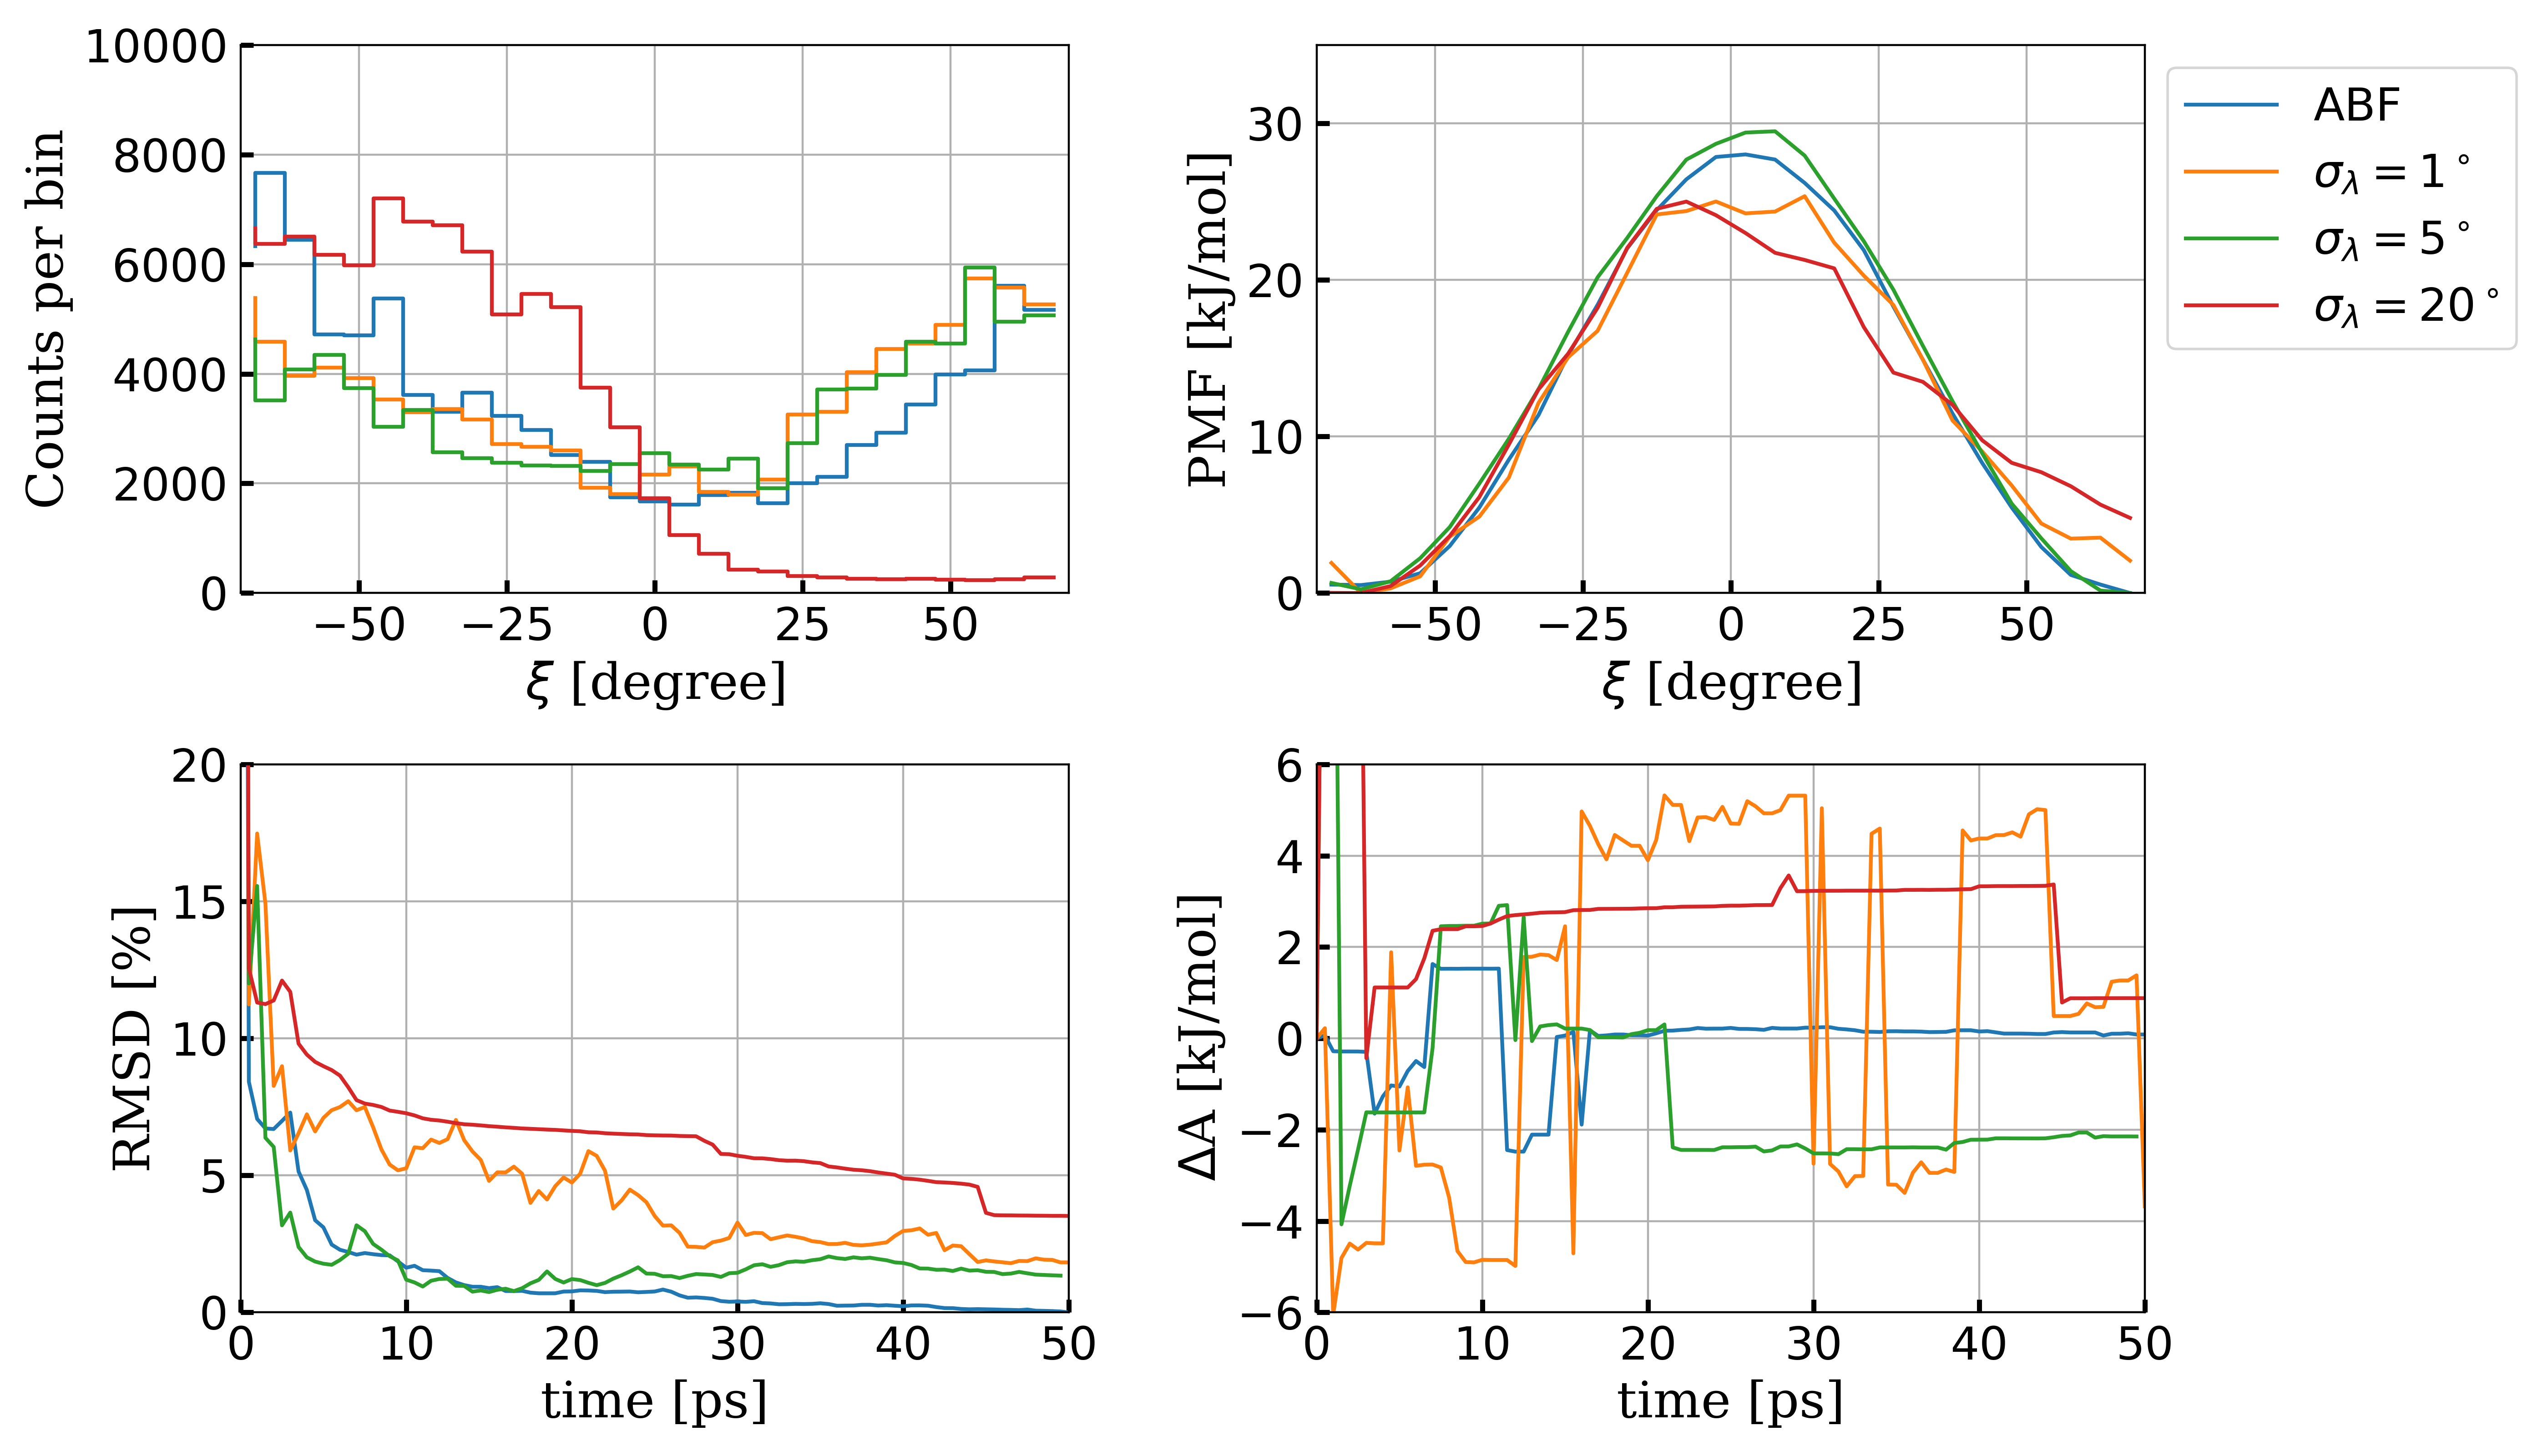
\includegraphics[width=0.99\textwidth]{bilder/benchmark/eABF_benchmark_sigma}
   \caption{Convergence of eABF with $m_\lambda=15$~a.u. and $N_{full}=100$.}
   \label{fig:conf eABF sigma}
\end{figure}

\begin{figure}[H]
  \centering
    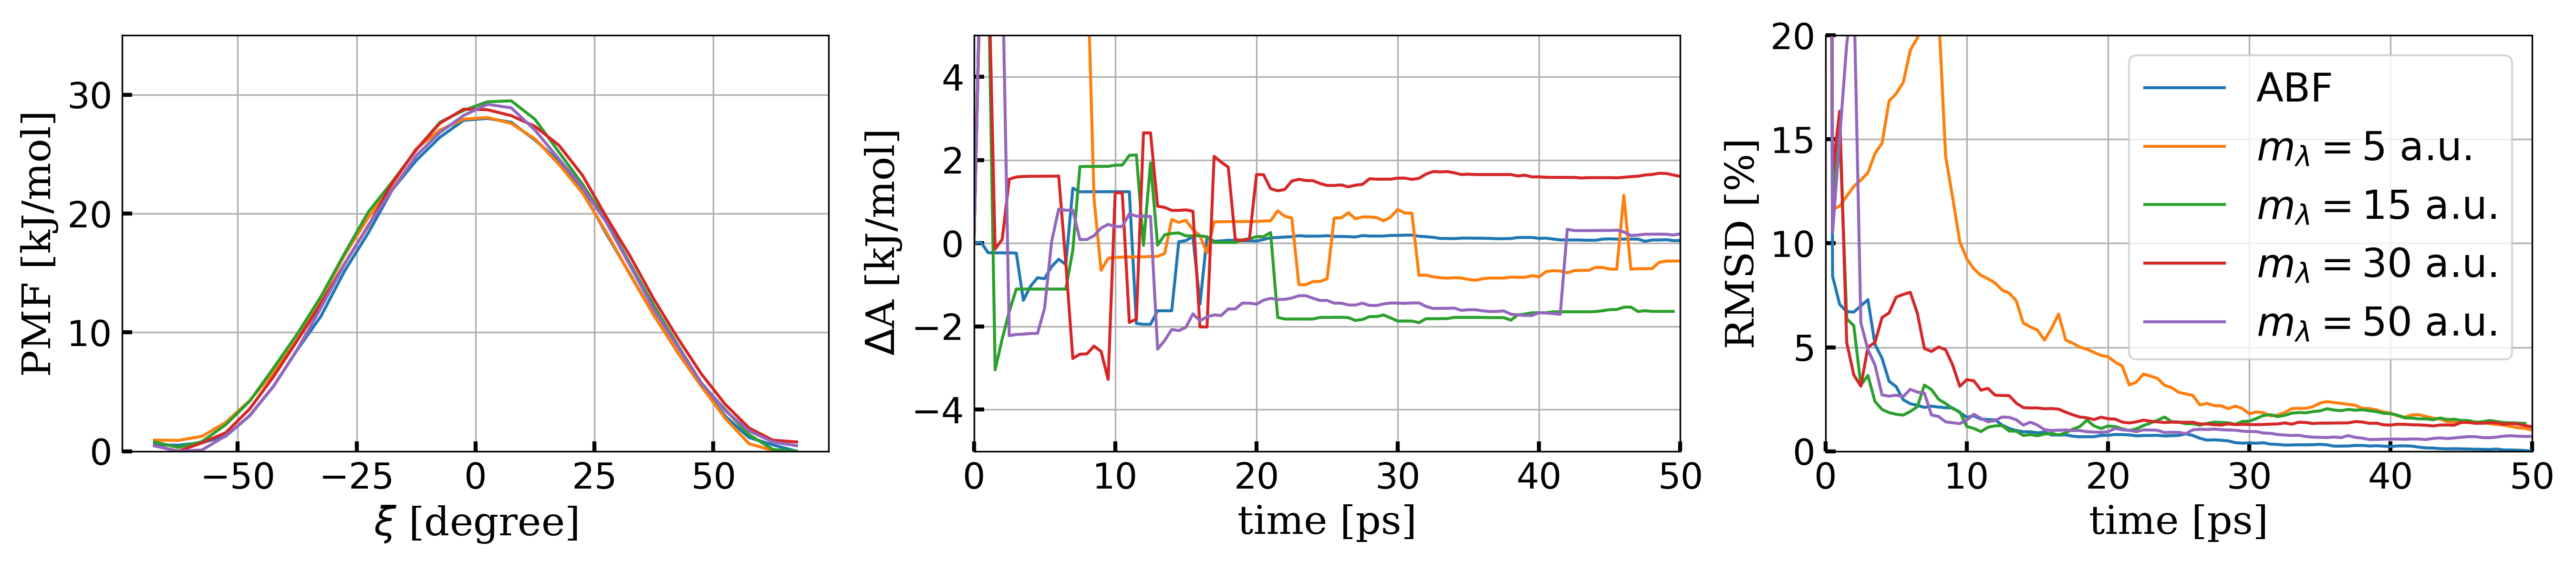
\includegraphics[width=0.99\textwidth]{bilder/benchmark/eABF_benchmark_mass}
   \caption{Convergence of eABF with $\sigma_\lambda=5$ degree and $N_{full}=100$.}
   \label{fig:conf eABF mass}
\end{figure}

\begin{figure}[H]
  \centering
    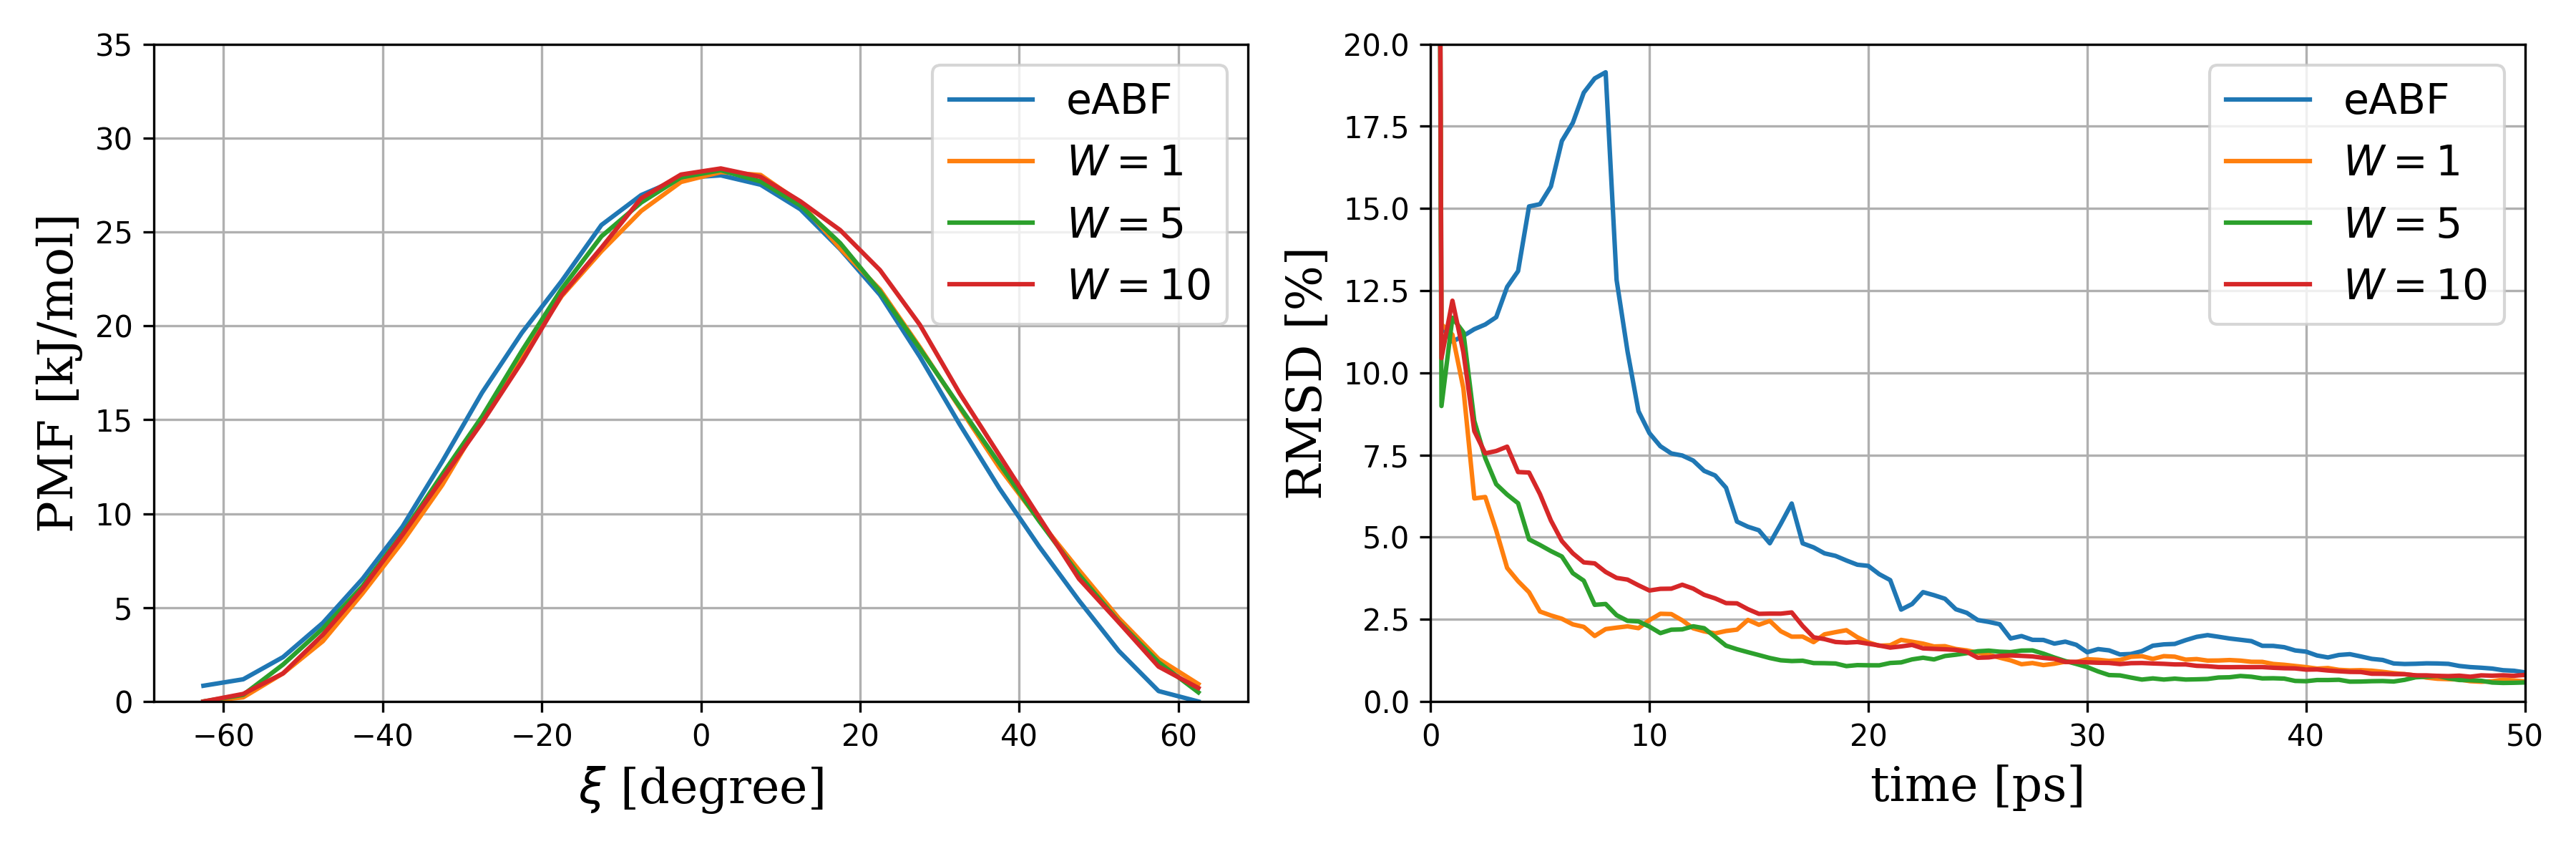
\includegraphics[width=0.99\textwidth]{bilder/benchmark/meta_eABF_benchmark_height}
   \caption{Convergence of WTM-eABF with $m_\lambda=5$~a.u., $\sigma_\lambda=5$, $\sigma_G=5$, $\tau_G=10$~fs, $\Delta T=2000$~K and $N_{full}=100$.}
   \label{fig:conf meABF height}
\end{figure}

\begin{figure}[H]
  \centering
    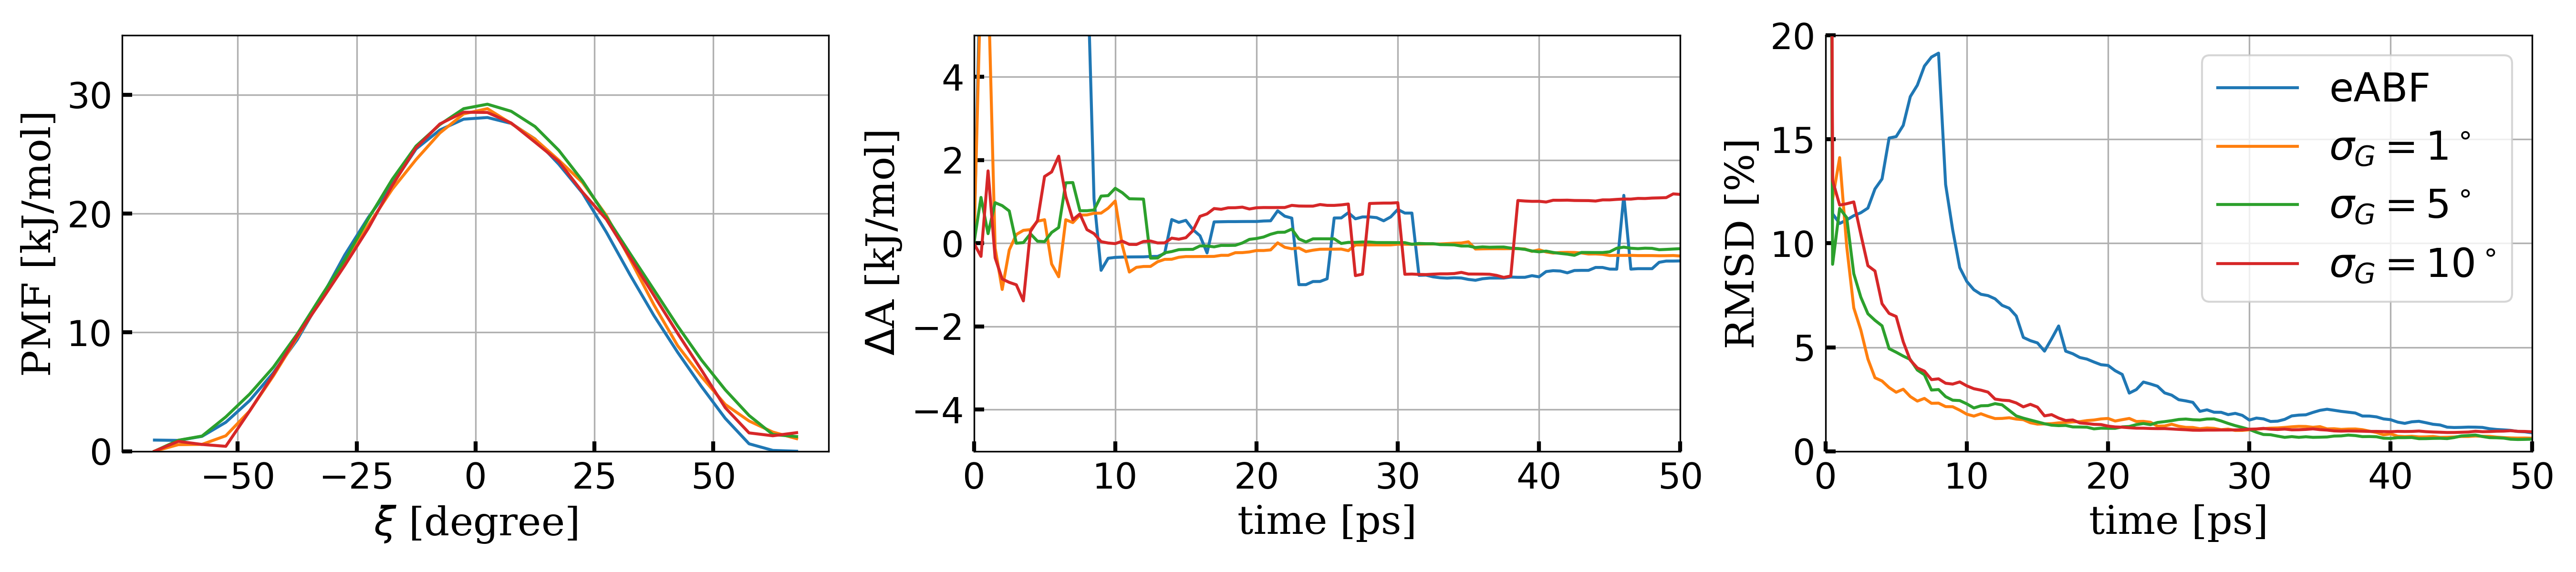
\includegraphics[width=0.99\textwidth]{bilder/benchmark/meta_eABF_benchmark_var}
   \caption{Convergence of WTM-eABF with $m_\lambda=5$~a.u., $\sigma_\lambda=5$, $W=5$ kJ/mol, $\tau_G=10$~fs, $\Delta T=2000$~K and $N_{full}=100$.}
   \label{fig:conf meABF var}
\end{figure}

% \begin{figure}[H]
%     \centering
%     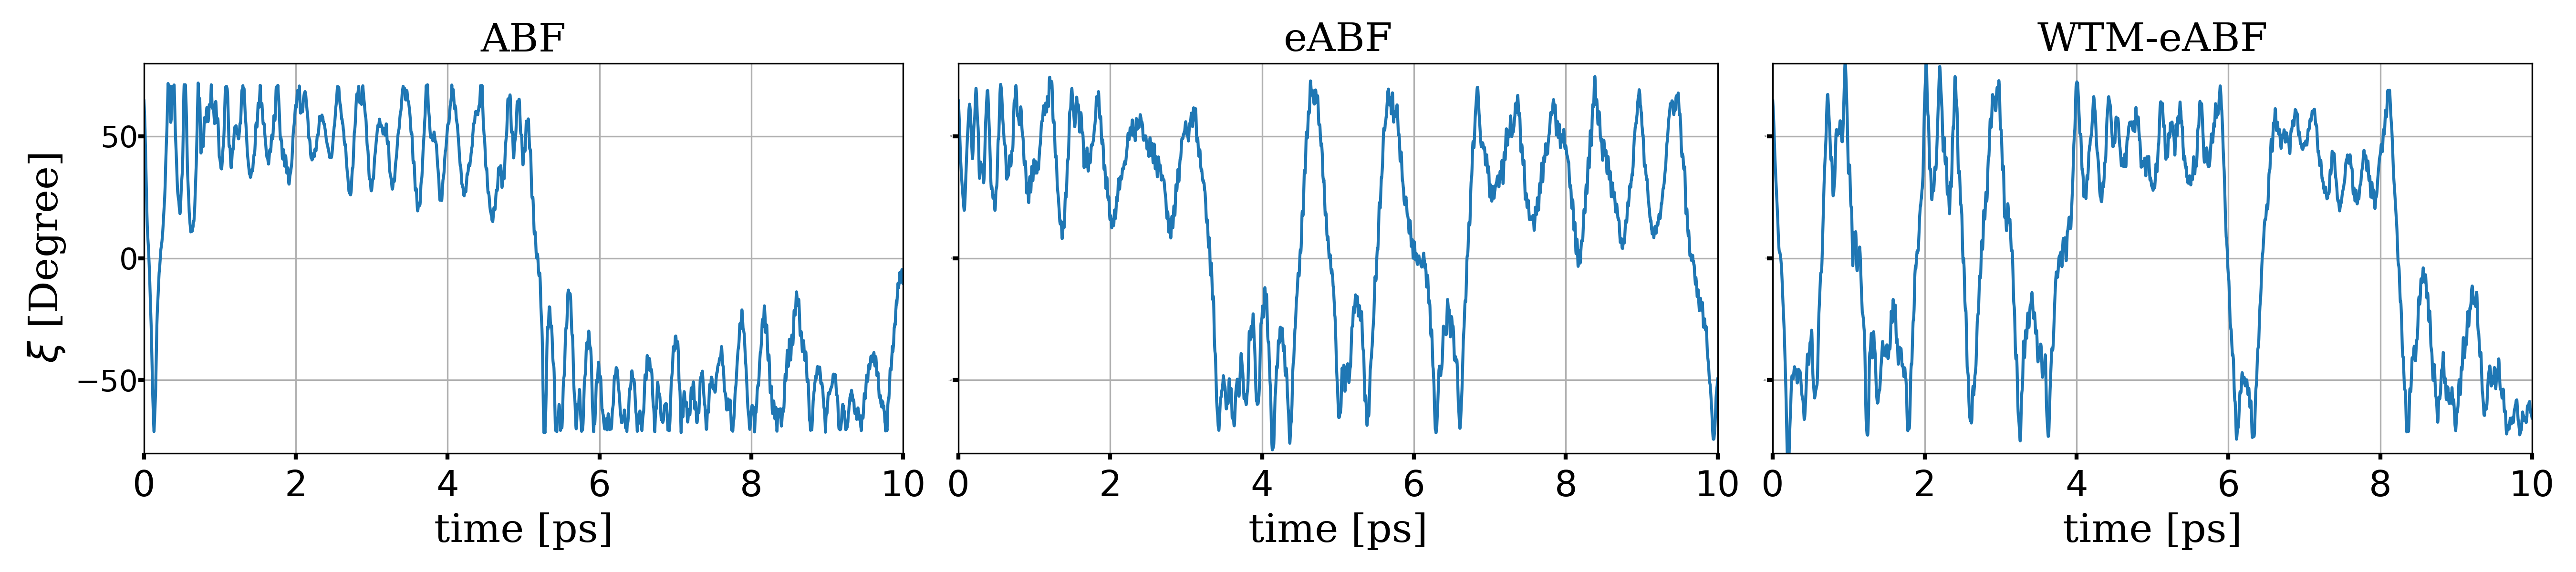
\includegraphics[width=0.99\textwidth]{bilder/benchmark/ABF_trajs}
%     \caption{Trajectories during ABF, eABF and WTM-eABF simulation.}
%     \label{fig:traj ABF}
% \end{figure}

\begin{figure}[H]
  \centering
    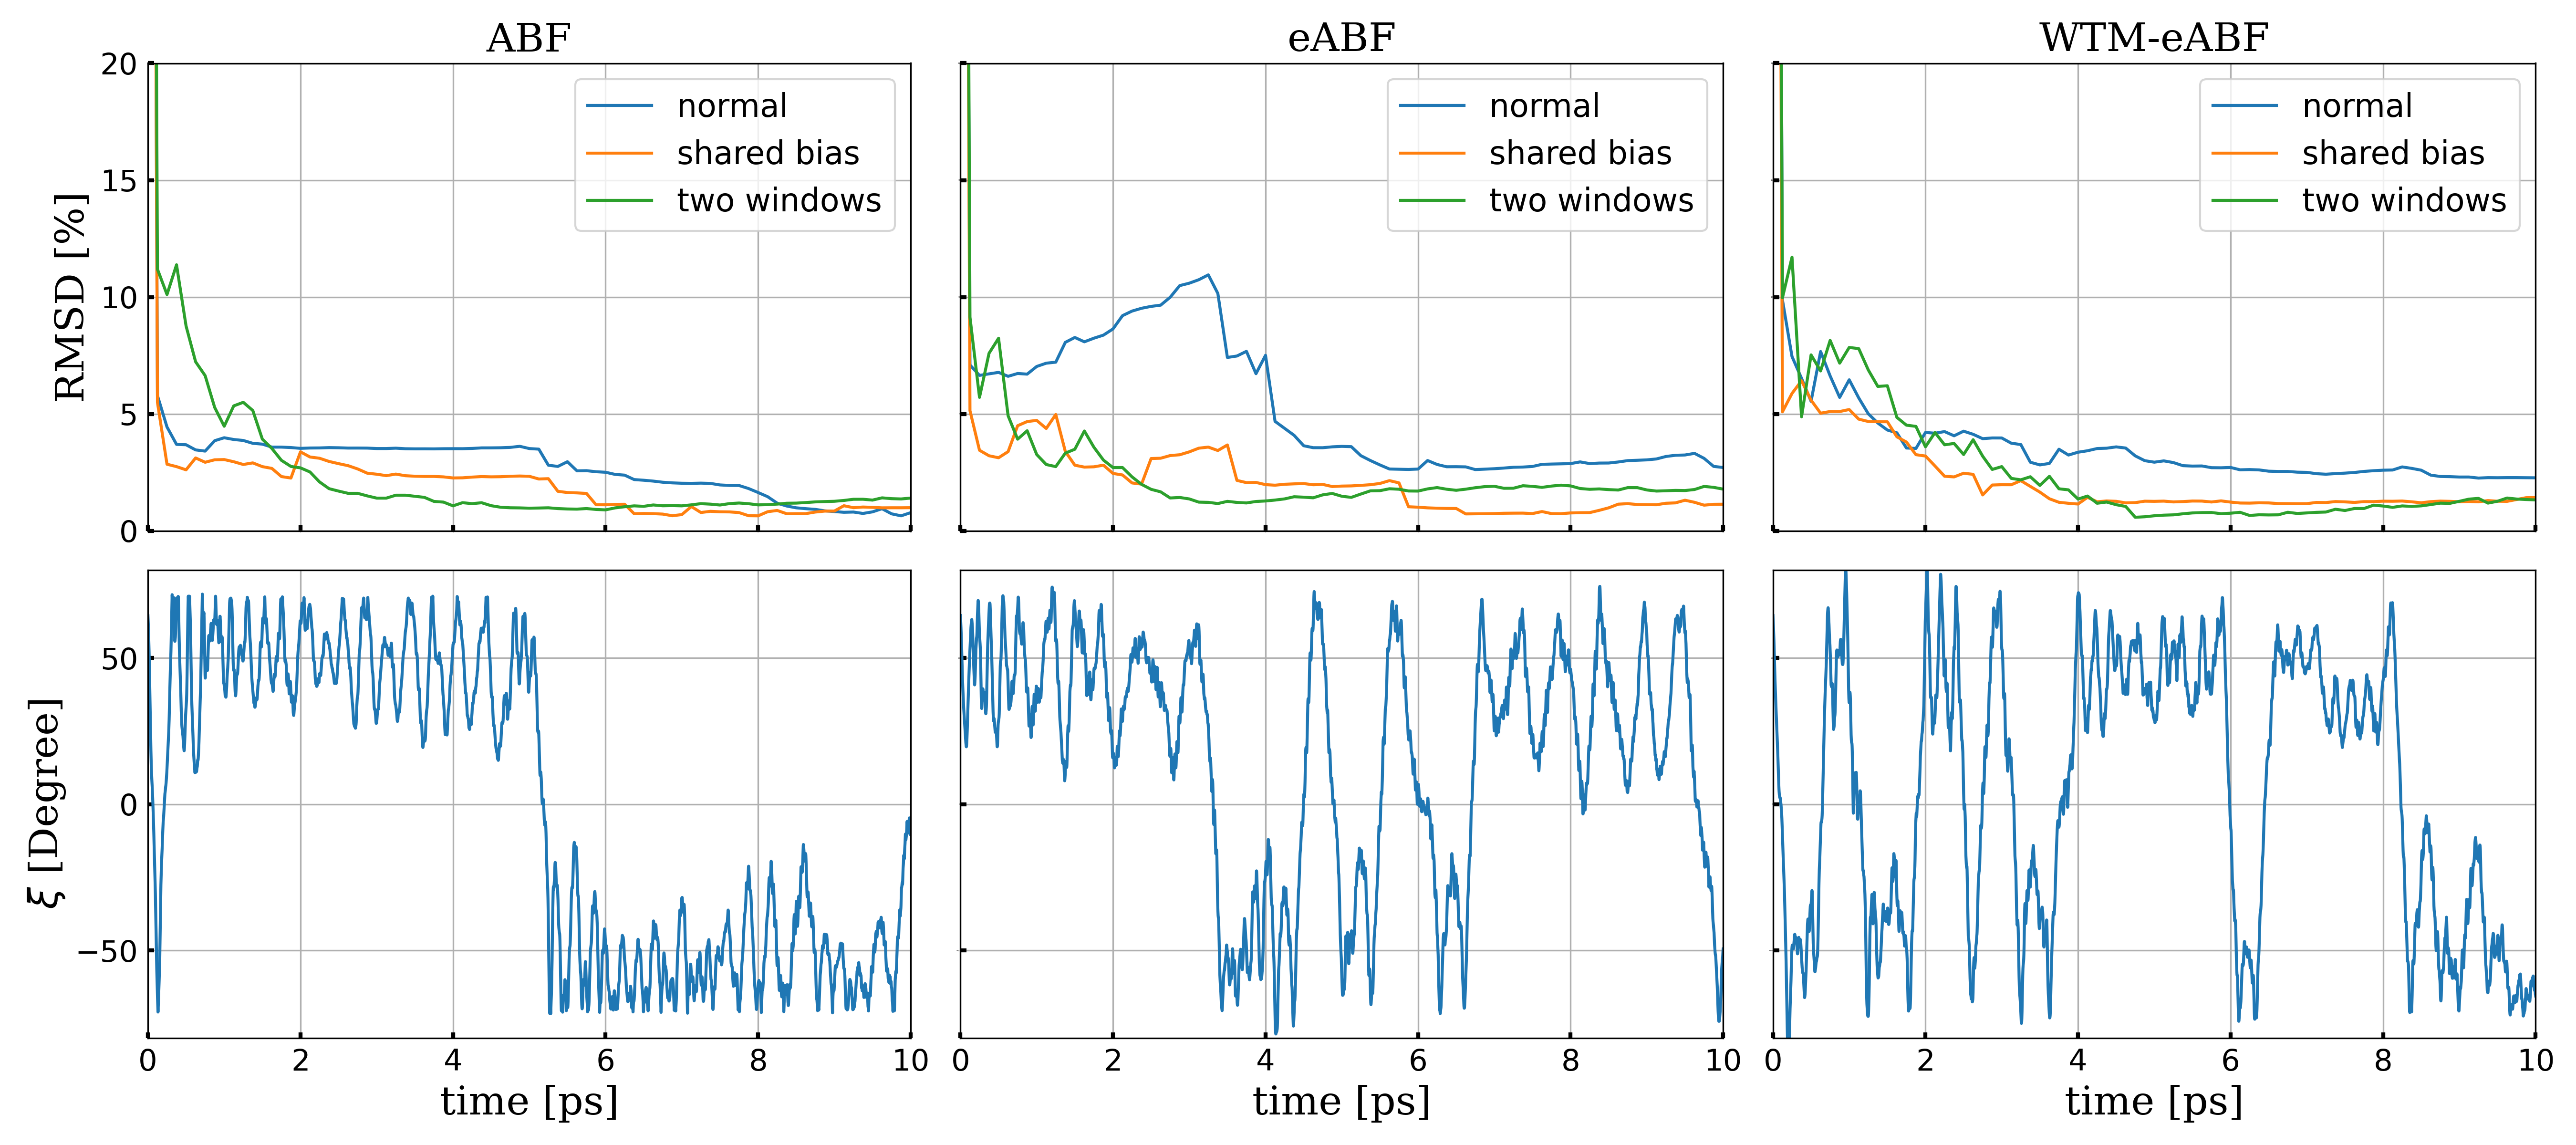
\includegraphics[width=0.99\textwidth]{bilder/benchmark/ABF_acc_benchmark}
   \caption{Convergence of ABF, eABF and WTM-eABF}
   \label{fig:conf ABF}
\end{figure}


% \begin{figure}[H]
%    \centering
%     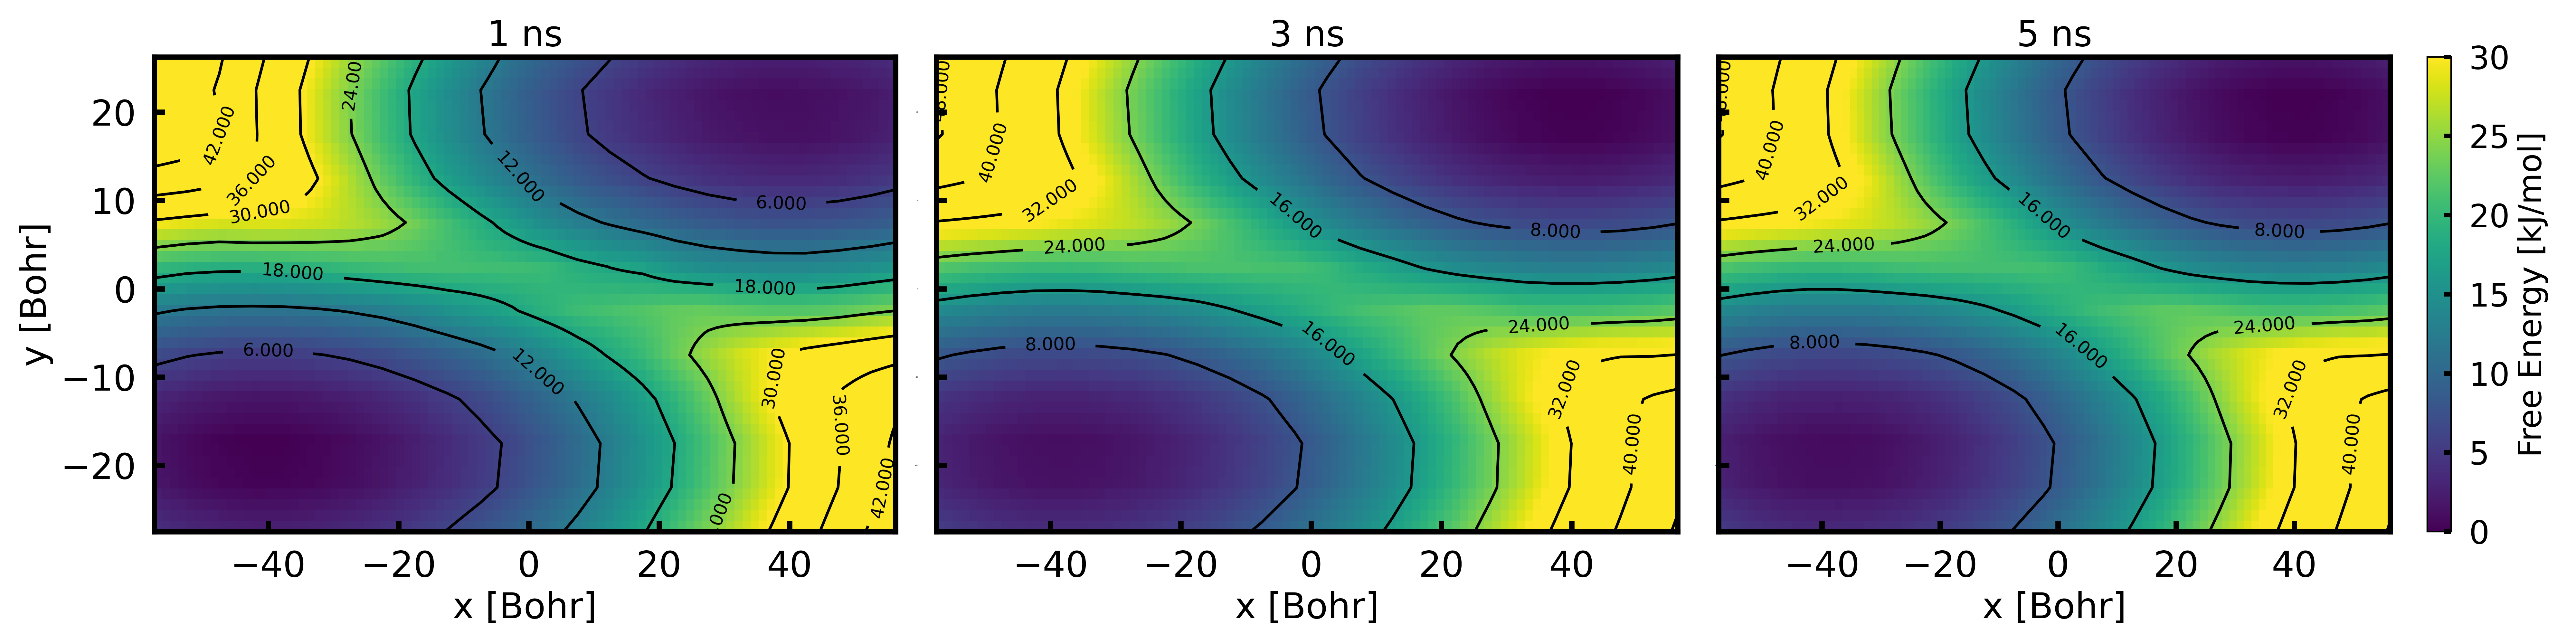
\includegraphics[width=0.99\textwidth]{bilder/test_2D/ABF}  \\
%     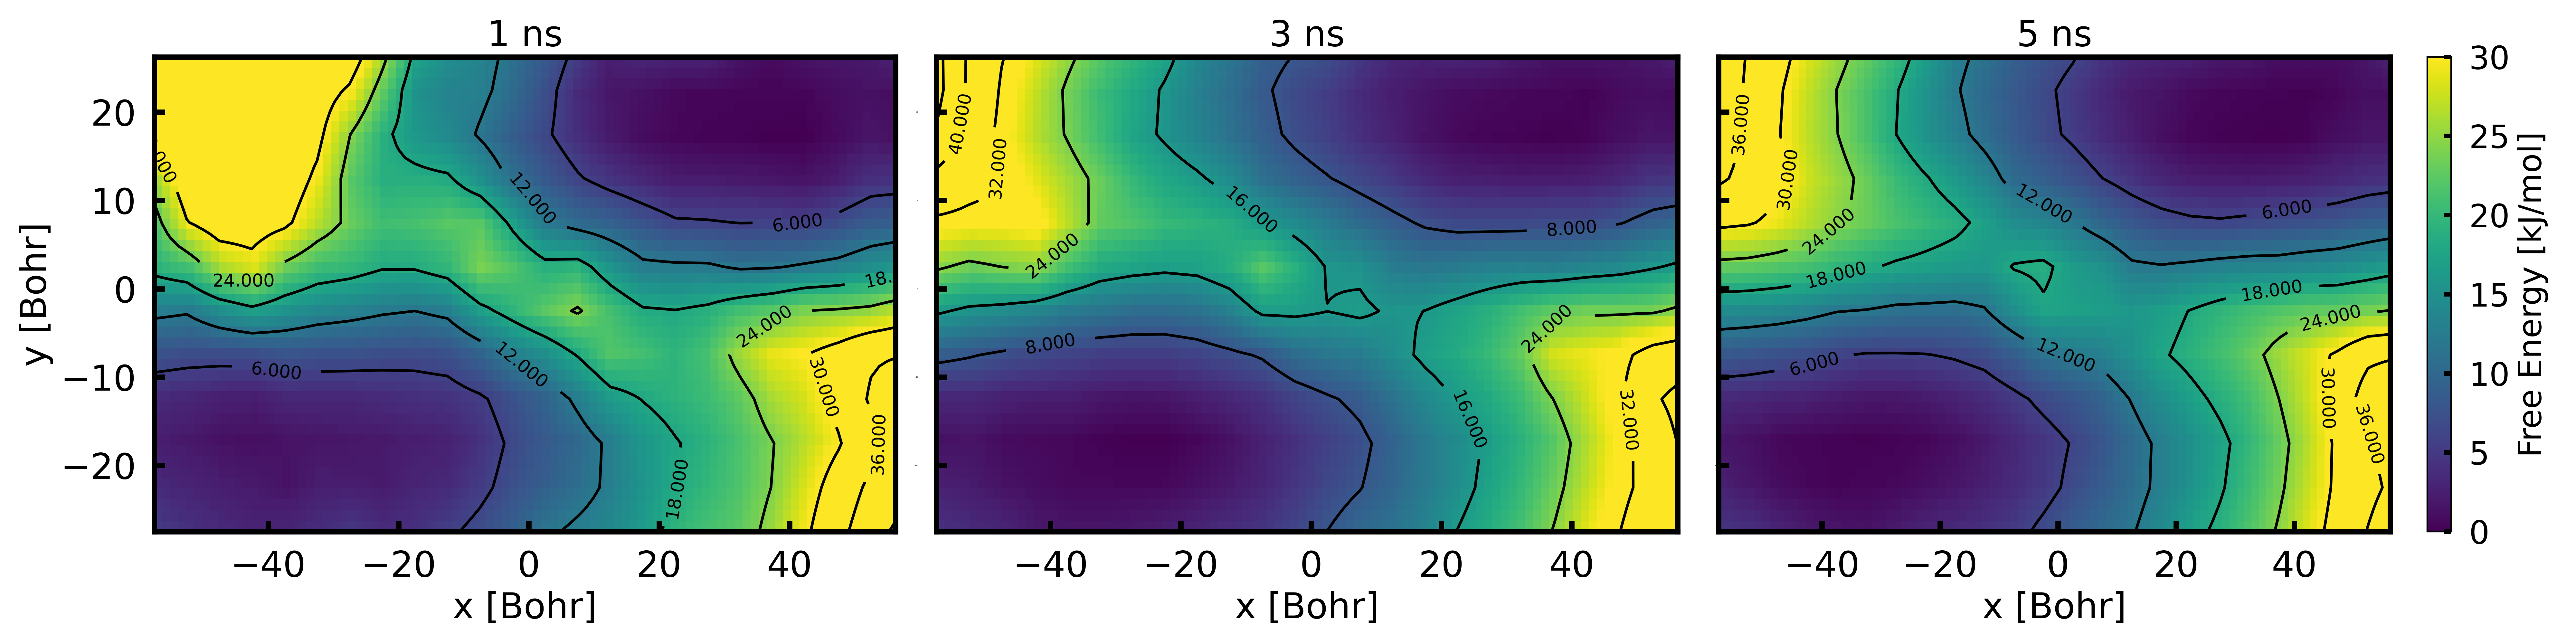
\includegraphics[width=0.99\textwidth]{bilder/test_2D/eABF} \\
%     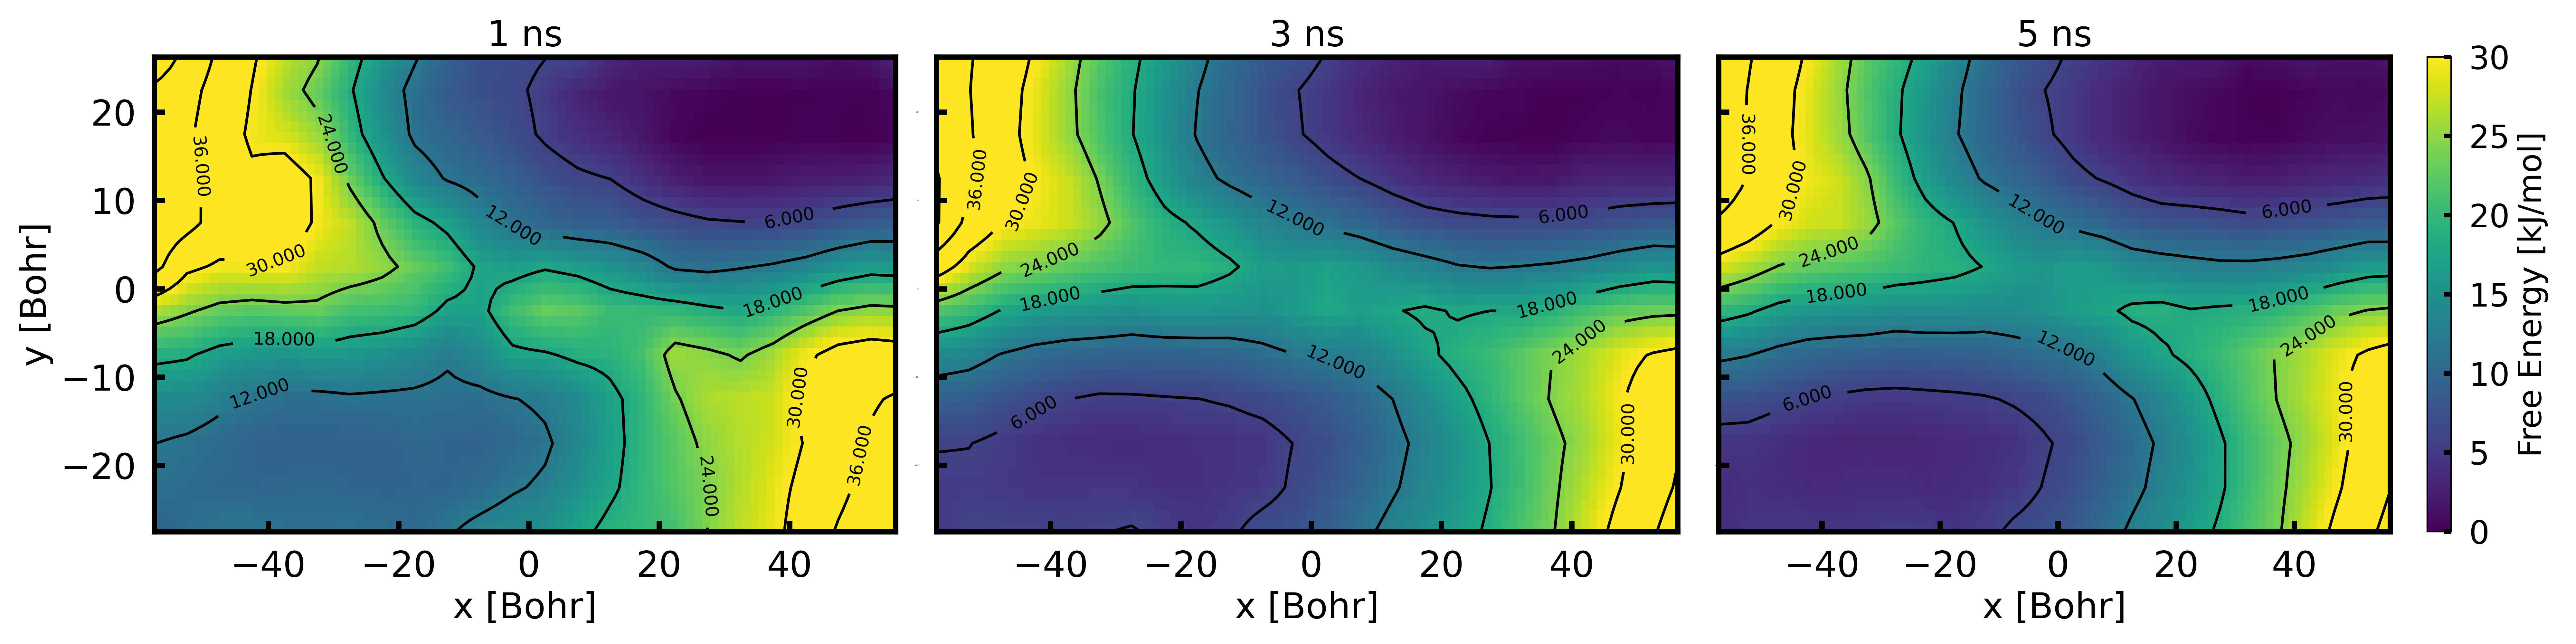
\includegraphics[width=0.99\textwidth]{bilder/test_2D/meta_eABF}
%     \caption{2D ABF, eABF and WTM-eABF test}
% \label{fig:2D ABF}%
% \end{figure}


\section{Application of WTM-eABF to S\textsubscript{n}2-Reactions}
\label{sec:Sn2}


\section{Ring Closing Reaction}
\label{sec:RCR}

\begin{figure}[H]
  \centering
    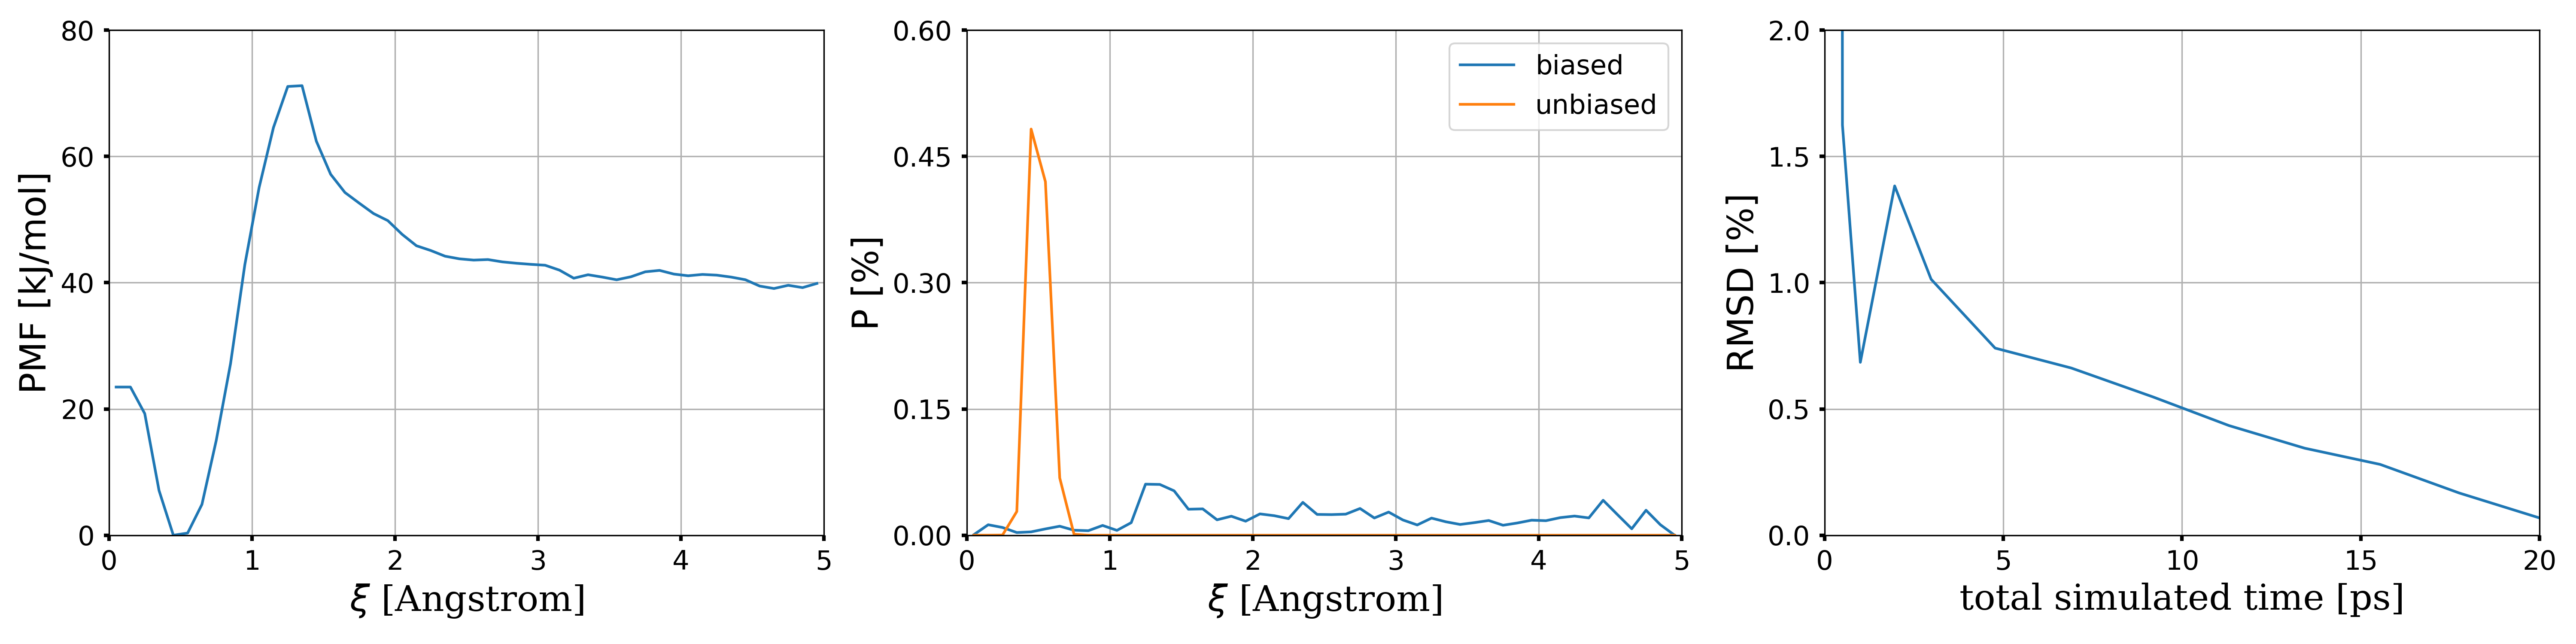
\includegraphics[width=0.99\textwidth]{bilder/results/R2_ool_results}
   \caption{Ring closing reaction}
   \label{fig:ool}
\end{figure}
